\documentclass[10pt]{beamer}

\usetheme{metropolis}

\usepackage{booktabs}
\usepackage{pgfplots}
\usepackage{listings}
\usepackage{xcolor}

\lstset{
	basicstyle=\ttfamily,
	frame=shadowbox,
	rulesepcolor=\color{gray},
	columns=fullflexible,
	commentstyle=\color{gray},
	keywordstyle=\bfseries\color{red},
	escapeinside={\%*}{*)},
  aboveskip=2em,
  captionpos=b,
  abovecaptionskip=1em,
  belowcaptionskip=1em
}

\title{Midway presentation}
\subtitle{Group 1}
\date{12 November 2018}
\author{Claudio Maggioni}
\titlegraphic{\centering{
\includegraphics[height=1cm]{logo.png}}}

\begin{document}

\maketitle

\begin{frame}[standout]
\centering{\Huge Slides in \LaTeX}
\end{frame}

\section{Progress up to now}

\begin{frame}[fragile]{Search box}
\vfill\centering{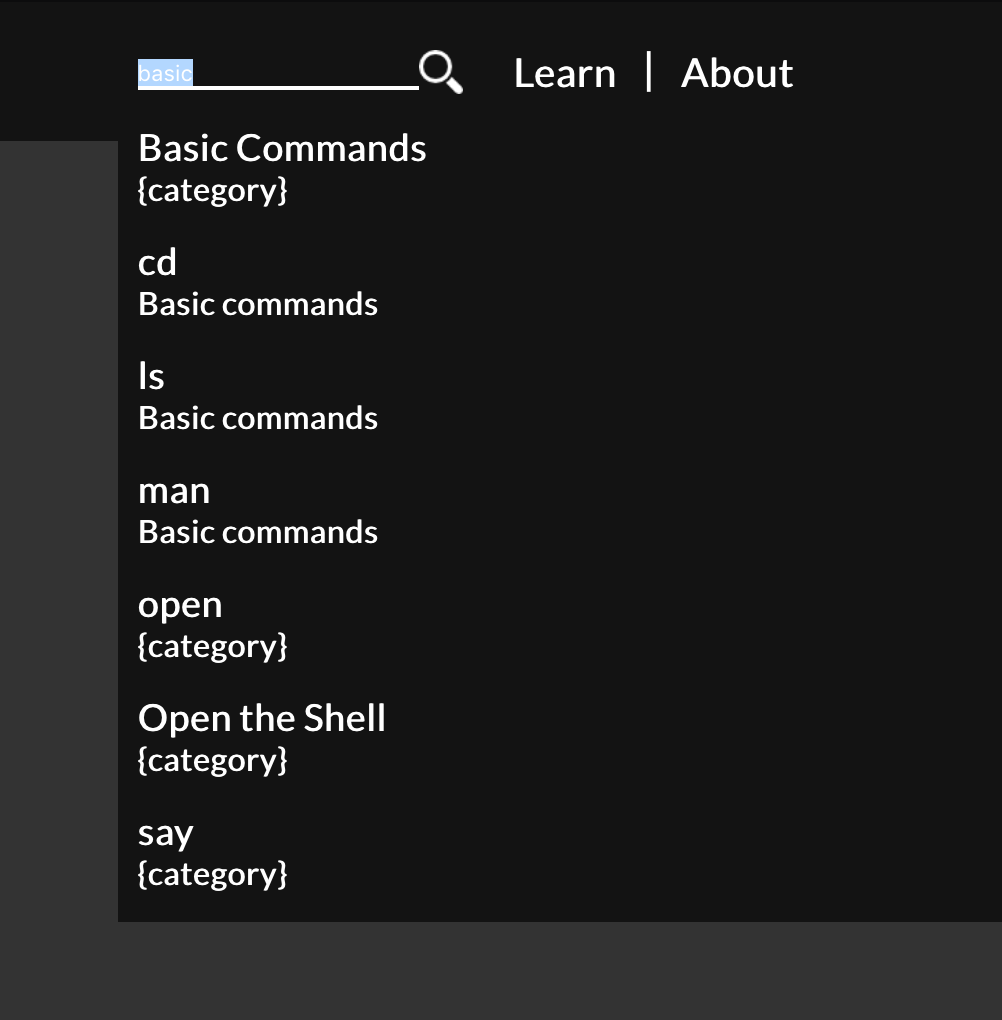
\includegraphics[width=0.6\textwidth]{search.png}}\vfill
\end{frame}

\begin{frame}[fragile]{Automatic topic index pages}
\vfill\centering{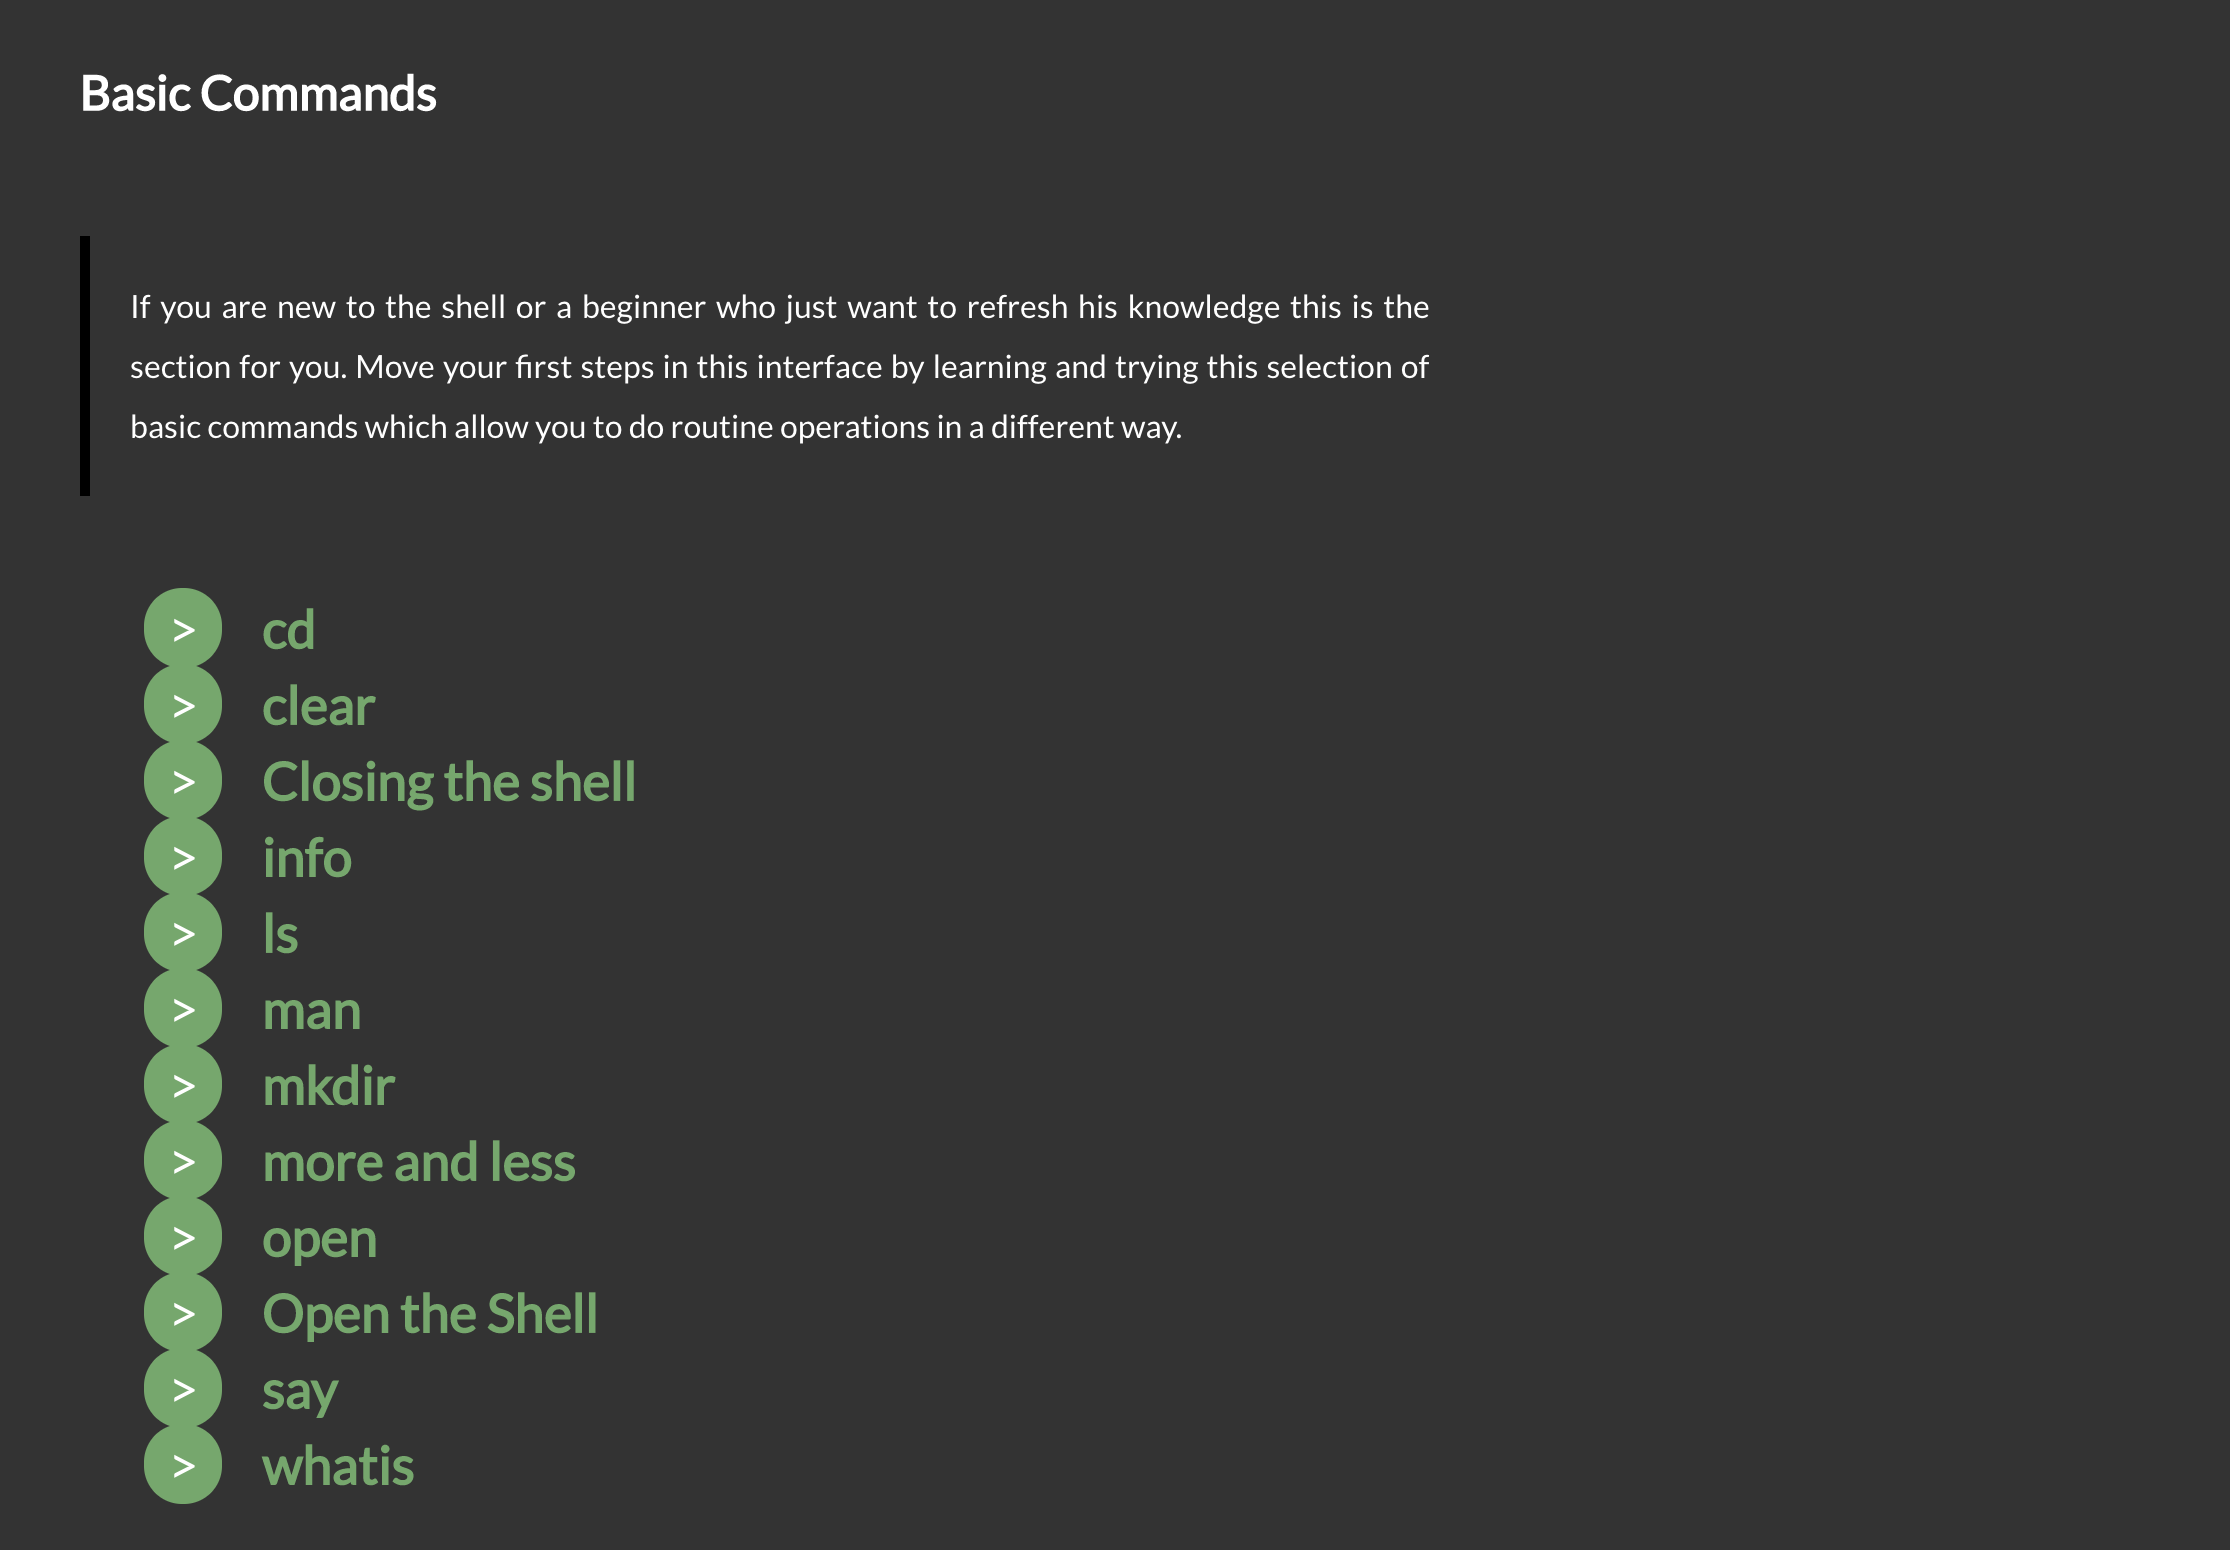
\includegraphics[width=0.6\textwidth]{index.png}}\vfill
\end{frame}

\begin{frame}[fragile]{Basic style}
\vfill\centering{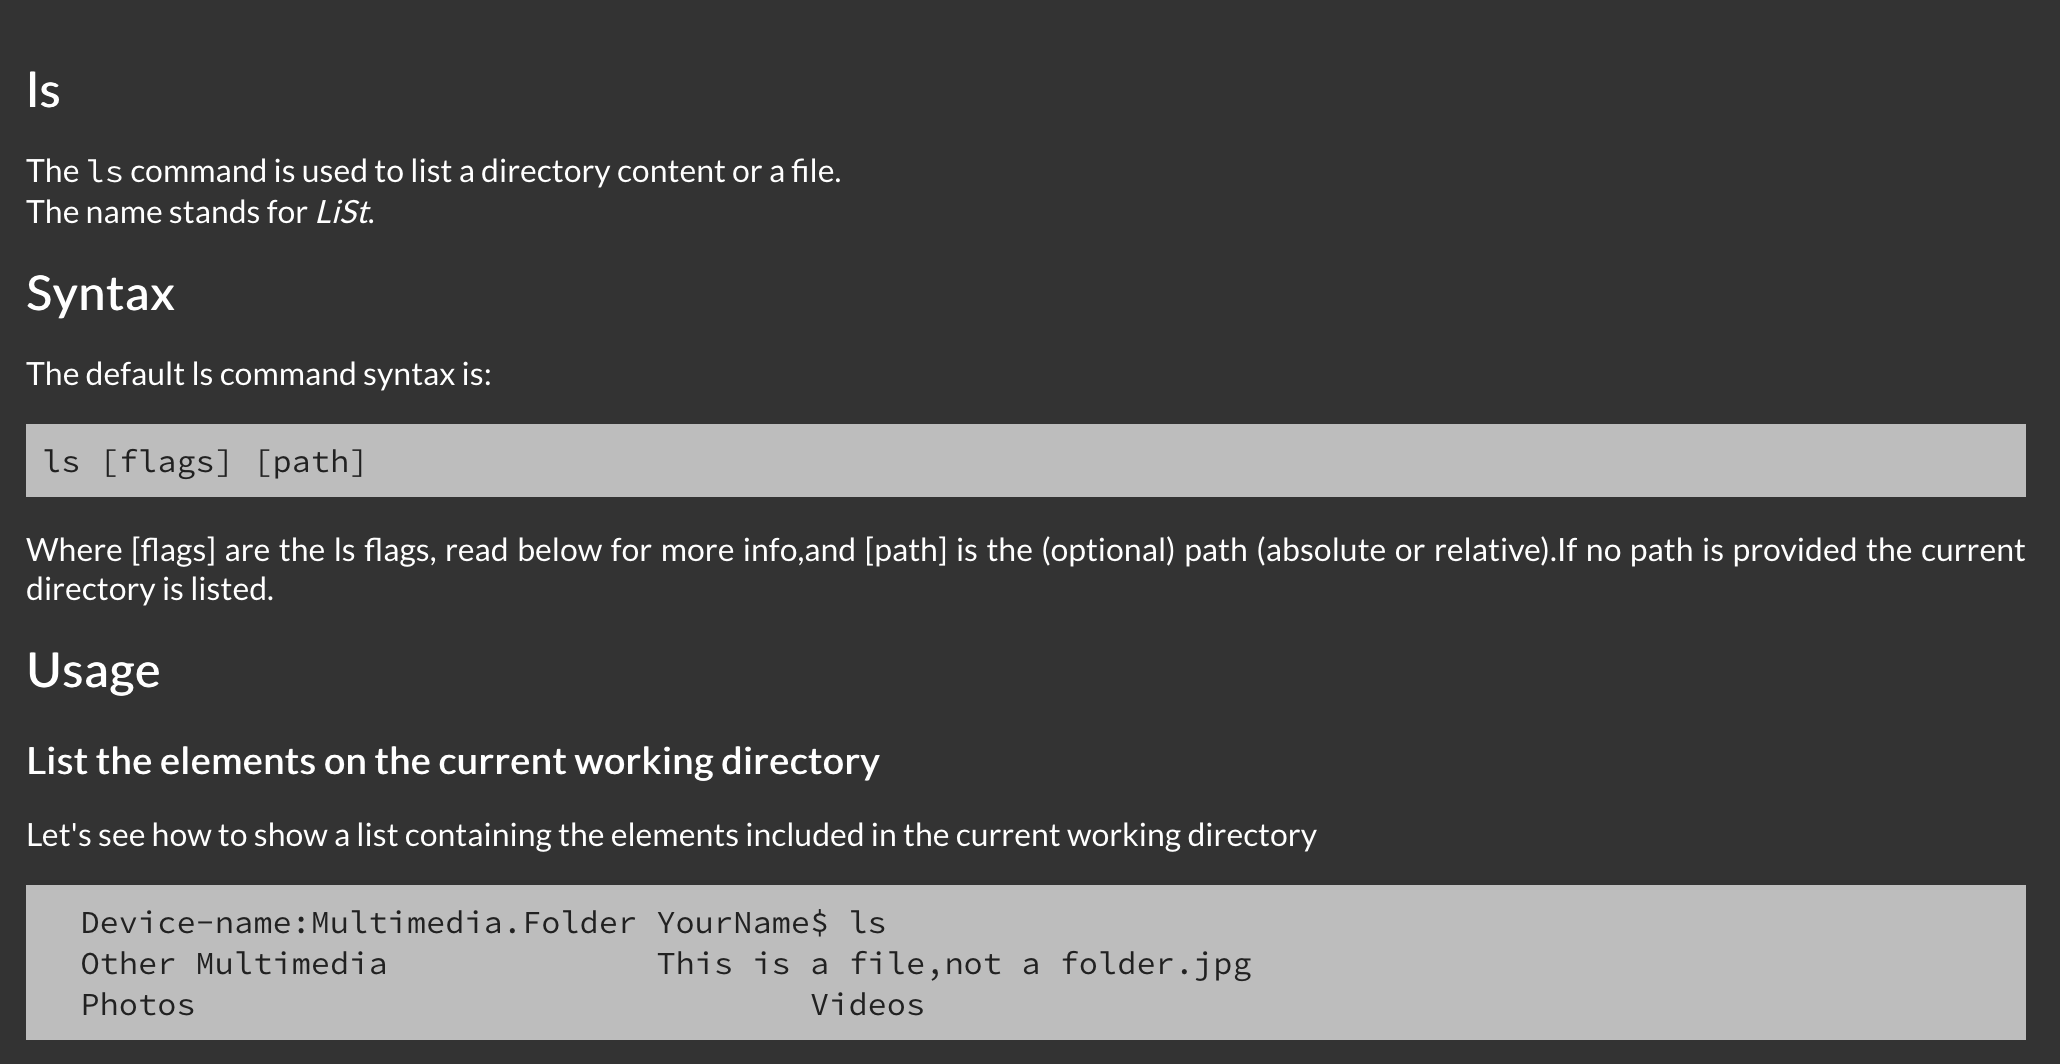
\includegraphics[width=\textwidth]{formatting.png}}\vfill
\end{frame}

\begin{frame}[fragile]{Automatic attribution (in footer)}
\vfill\centering{
\includegraphics[width=0.8\textwidth]{footer.png}}\vfill
\end{frame}

\begin{frame}[fragile]{Automatic attribution (in about page)}
\vfill\centering{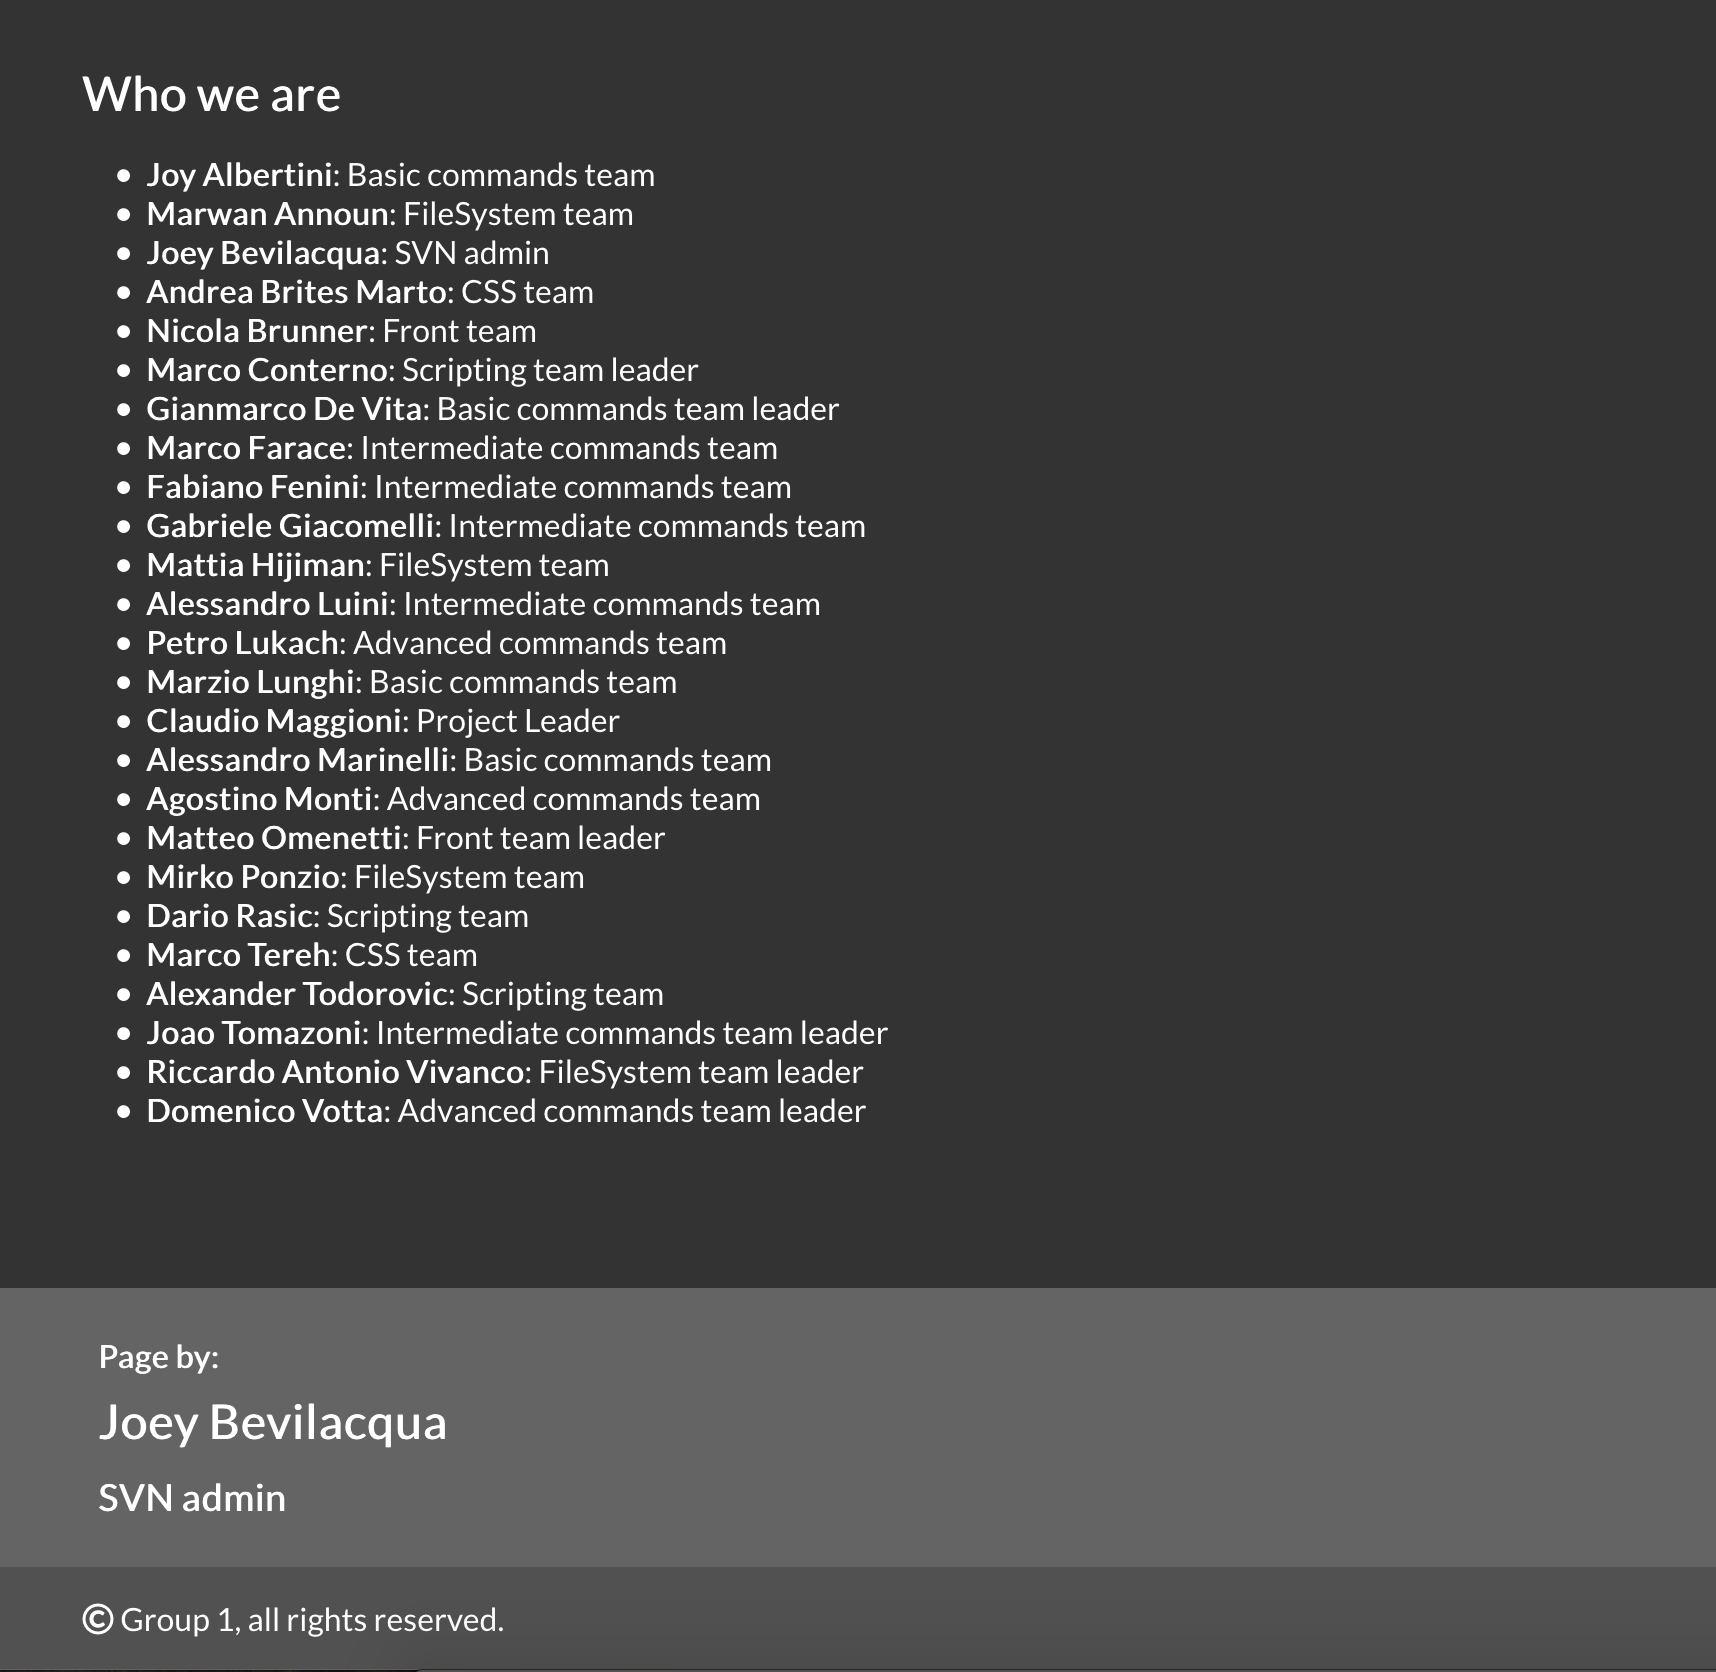
\includegraphics[width=0.7\textwidth]{about.png}}\vfill
\end{frame}

\begin{frame}[fragile]{Bonus 1 almost done}
\vfill\centering{
\includegraphics[width=0.7\textwidth]{rust.png}}\vfill
\end{frame}

\begin{frame}[standout]
\centering{\Huge Nystrom seal of quality}
\end{frame}

\section{First code review for content}

\begin{frame}[fragile]{A properly formatted Jekyll page}
\begin{figure}[h]
\begin{lstlisting}[language=html,basicstyle=\small\ttfamily]
---
layout: page
category-title: Basic commands
category-page: basic
tags: directory list
author: Claudio Maggioni
title: ls
---
<p>The <code>ls</code> command is used to list a
directory content or a file.<br>
The name stands for <i>LiSt</i>.

<h2>Usage</h2>
<p>...</p>
\end{lstlisting}
\end{figure}
\end{frame}

{\setbeamercolor{background canvas}{bg=black}
\begin{frame}
\centering{\Huge\fontspec{Comic Sans MS}\color{red} 
	\textsc{The evil side of HTML \\
	\vspace{0.5cm}
	(and Jekyll)}}
\end{frame}}

\begin{frame}[fragile]
\begin{figure}[h]
\begin{lstlisting}[language=html]
title: ...
...
---

<html>
<head>
</head>

<body>
<header>

<h1>...</h1>
...
</header>
</body>
</html>
\end{lstlisting}
\end{figure}
\end{frame}

\begin{frame}[fragile]
\begin{figure}[h]
\begin{lstlisting}[language=html]
<div class="title1">
    <h1>...</h1>
</div>

A list of things:
<br> ...
<br> ...
<br> ...
<br> ...
<br> ...
\end{lstlisting}
\end{figure}
\end{frame}

\begin{frame}[fragile]
\begin{figure}[h]
\begin{lstlisting}[language=html]
<!-- No Jekyll header -->

<!DOCTYPE html>
...
\end{lstlisting}
\end{figure}
\end{frame}

\begin{frame}{Page creation guide}
\vfill\centering{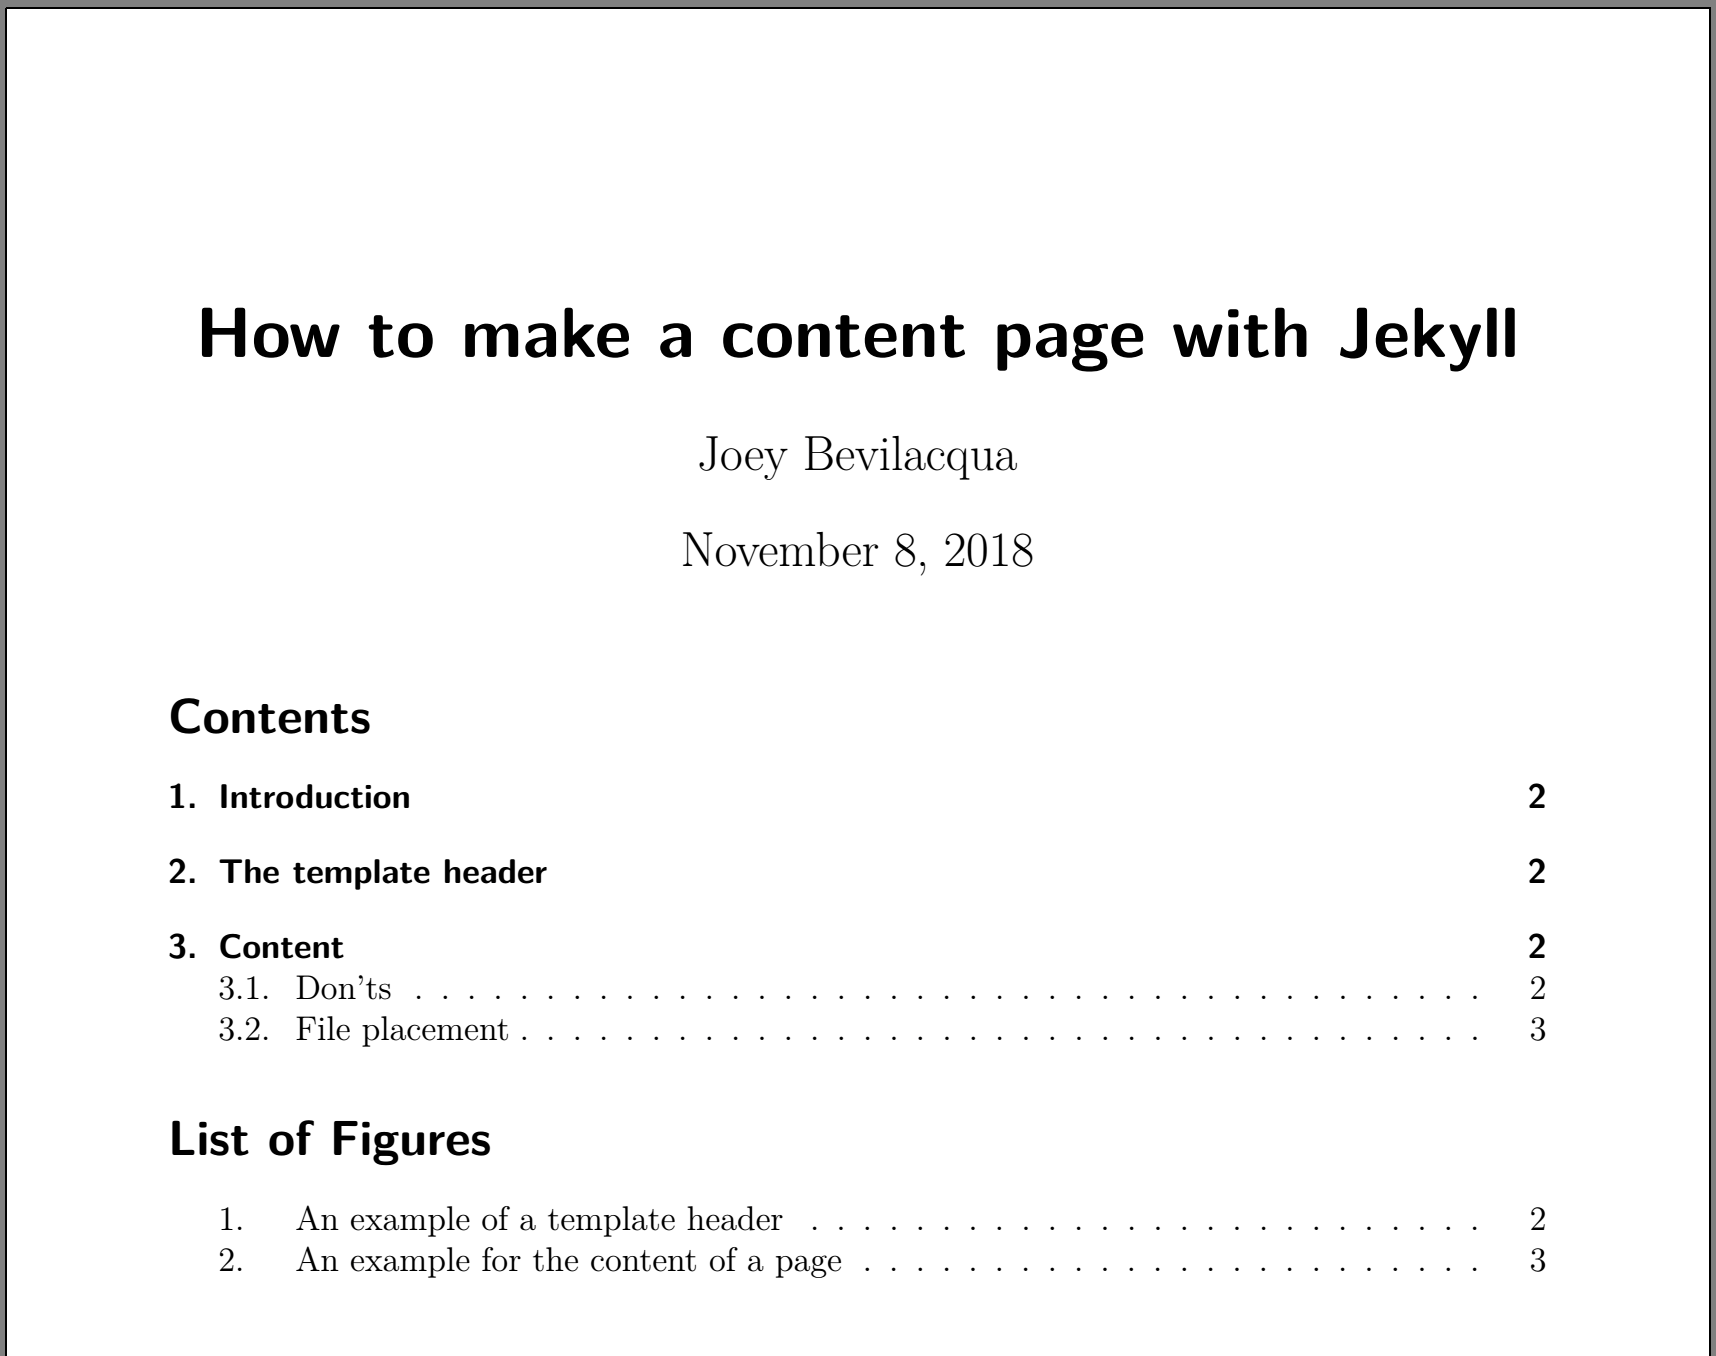
\includegraphics[width=0.8\textwidth]{page_creation.png}}\vfill
\end{frame}

\section{Code contribution}

\begin{frame}[fragile]{LOC stats}
\begin{lstlisting}[language=bash]
svn ls -R | egrep -v -e "\/\$" | xargs svn blame \
    | awk '{print $2}' | sort | uniq -c | sort -r
\end{lstlisting}
\vfill
This is not accurate:
\begin{itemize}
\item Only text files considered, not images or videos
\item Assumes each person commits with their own user
\item Writing 2 lines of complex code doesn't take the same time as writing 2 lines from a documentation
\end{itemize}
\end{frame}

\begin{frame}{LOC stats (as of 2018-11-12 12:00)}
\begin{figure}
    \begin{tikzpicture}
      \begin{axis}[
        legend pos=north east,
        mbarplot,
        enlarge x limits={0.5},
        symbolic x coords={LOC},
        width=\textwidth,
        height=8.5cm,
        xtick=data
      ]
      
      \legend{maggicl, bevilj, britea, vottad, devitg, annoum, brunnn, terehm, luinia,
      	rasicd, ponzim, feninif, marina, hijmam, omenem}

      \addplot plot coordinates {(LOC,2405)};
      \addplot plot coordinates {(LOC,978)};
      \addplot plot coordinates {(LOC,171)};
      \addplot plot coordinates {(LOC,145)};
      \addplot plot coordinates {(LOC,144)};
      \addplot plot coordinates {(LOC,130)};
      \addplot plot coordinates {(LOC,128)};
      \addplot plot coordinates {(LOC,116)};
      \addplot plot coordinates {(LOC,108)};
      \addplot plot coordinates {(LOC,85)};
      \addplot plot coordinates {(LOC,66)};
      \addplot plot coordinates {(LOC,63)};
      \addplot plot coordinates {(LOC,36)};
      \addplot plot coordinates {(LOC,36)}; 
      \addplot plot coordinates {(LOC,22)};     
      \addplot plot coordinates {(LOC,22)};
      \addplot plot coordinates {(LOC,13)};
      \end{axis}
    \end{tikzpicture}
  \end{figure}
\end{frame}

\begin{frame}[standout]
\centering{\Huge Demo time!}
\end{frame}

\end{document}
